% ========================================
%	Header einbinden
% ========================================

\documentclass[bibtotoc,titlepage]{scrartcl}

% Deutsche Spracheinstellungen
\usepackage[ngerman,german]{babel, varioref}
\usepackage[T1]{fontenc}
\usepackage[utf8]{inputenc}

%\usepackage{marvosym}

\usepackage{amsfonts}
\usepackage{amssymb}
\usepackage{amsmath}
\usepackage{amscd}
\usepackage{amstext}

\usepackage{longtable}

%\usepackage{bibgerm}

\usepackage{footnpag}

\usepackage{ifthen}                 %%% package for conditionals in TeX
\usepackage[amssymb]{SIunits}
%Für textumflossene Bilder und Tablellen
%\usepackage{floatflt} - veraltet

%Für Testzwecke aktivieren, zeigt labels und refs im Text an.
%\usepackage{showkeys}

% Abstand zwischen zwei Absätzen nach DIN (1,5 Zeilen)
% \setlength{\parskip}{1.5ex plus0.5ex minus0.5ex}

% Einrückung am Anfang eines neuen Absatzes nach DIN (keine)
%\setlength{\parindent}{0pt}

% Ränder definieren
% \setlength{\oddsidemargin}{0.3cm}
% \setlength{\textwidth}{15.6cm}

% bessere Bildunterschriften
%\usepackage[center]{caption2}


% Problemlösungen beim Umgang mit Gleitumgebungen
\usepackage{float}

% Nummeriert bis zur Strukturstufe 3 (also <section>, <subsection> und <subsubsection>)
%\setcounter{secnumdepth}{3}

% Führt das Inhaltsverzeichnis bis zur Strukturstufe 3
%\setcounter{tocdepth}{3}
\usepackage[version=3]{mhchem}
	\mhchemoptions{minus-sidebearing-left=0.06em, minus-sidebearing-right=0.11em}
\usepackage{exscale}

\newenvironment{dsm} {\begin{displaymath}} {\end{displaymath}}
\newenvironment{vars} {\begin{center}\scriptsize} {\normalsize \end{center}}


\newcommand {\en} {\varepsilon_0}               % Epsilon-Null aus der Elektrodynamik
\newcommand {\lap} {\; \mathbf{\Delta}}         % Laplace-Operator
\newcommand {\R} { \mathbb{R} }                 % Menge der reellen Zahlen
\newcommand {\e} { \ \mathbf{e} }               % Eulersche Zahl
\renewcommand {\i} { \mathbf{i} }               % komplexe Zahl i
\newcommand {\N} { \mathbb{N} }                 % Menge der nat. Zahlen
\newcommand {\C} { \mathbb{C} }                 % Menge der kompl. Zahlen
\newcommand {\Z} { \mathbb{Z} }                 % Menge der kompl. Zahlen
\newcommand {\limi}[1]{\lim_{#1 \rightarrow \infty}} % Limes unendlich
\newcommand {\sumi}[1]{\sum_{#1=0}^\infty}
\newcommand {\rot} {\; \mathrm{rot} \,}         % Rotation
\newcommand {\grad} {\; \mathrm{grad} \,}       % Gradient
\newcommand {\dive} {\; \mathrm{div} \,}        % Divergenz
\newcommand {\dx} {\; \mathrm{d} }              % Differential d
\newcommand {\cotanh} {\; \mathrm{cotanh} \,}   %Cotangenshyperbolicus
\newcommand {\asinh} {\; \mathrm{areasinh} \,}  %Area-Sinus-Hyp.
\newcommand {\acosh} {\; \mathrm{areacosh} \,}  %Area-Cosinus-H.
\newcommand {\atanh} {\; \mathrm{areatanh} \,}  %Area Tangens-H.
\newcommand {\acoth} {\; \mathrm{areacoth} \,}  % Area-cotangens
\newcommand {\Sp} {\; \mathrm{Sp} \,}
\newcommand {\mbe} {\stackrel{\text{!}}{=}}     %Must Be Equal
\newcommand{\qed} { \hfill $\square$\\}
\renewcommand{\i} {\imath}
\def\captionsngerman{\def\figurename{\textbf{Abb.}}}

%%%%%%%%%%%%%%%%%%%%%%%%%%%%%%%%%%%%%%%%%%%%%%%%%%%%%%%%%%%%%%%%%%%%%%%%%%%%
% SWITCH FOR PDFLATEX or LATEX
%%%%%%%%%%%%%%%%%%%%%%%%%%%%%%%%%%%%%%%%%%%%%%%%%%%%%%%%%%%%%%%%%%%%%%%%%%%%
%%%
\ifx\pdfoutput\undefined %%%%%%%%%%%%%%%%%%%%%%%%%%%%%%%%%%%%%%%%% LATEX %%%
%%%
\usepackage[dvips]{graphicx}       %%% graphics for dvips
\DeclareGraphicsExtensions{.eps,.ps}   %%% standard extension for included graphics
\usepackage[ps2pdf]{thumbpdf}      %%% thumbnails for ps2pdf
\usepackage[ps2pdf,                %%% hyper-references for ps2pdf
bookmarks=true,%                   %%% generate bookmarks ...
bookmarksnumbered=true,%           %%% ... with numbers
hypertexnames=false,%              %%% needed for correct links to figures !!!
breaklinks=true,%                  %%% breaks lines, but links are very small
linkbordercolor={0 0 1},%          %%% blue frames around links
pdfborder={0 0 112.0}]{hyperref}%  %%% border-width of frames
%                                      will be multiplied with 0.009 by ps2pdf
%
\hypersetup{ pdfauthor   = {Hannes Franke; Julius Tilly},
pdftitle    = {V301 Innenwiderstand und Leistungsanpassung}, pdfsubject  = {Protokoll FP}, pdfkeywords = {V301, Innenwiderstand, Leistungsanpassung},
pdfcreator  = {LaTeX with hyperref package}, pdfproducer = {dvips
+ ps2pdf} }
%%%
\else %%%%%%%%%%%%%%%%%%%%%%%%%%%%%%%%%%%%%%%%%%%%%%%%%%%%%%%%%% PDFLATEX %%%
%%%
\usepackage[pdftex]{graphicx}      %%% graphics for pdfLaTeX
\DeclareGraphicsExtensions{.pdf}   %%% standard extension for included graphics
\usepackage[pdftex]{thumbpdf}      %%% thumbnails for pdflatex
\usepackage[pdftex,                %%% hyper-references for pdflatex
bookmarks=true,%                   %%% generate bookmarks ...
bookmarksnumbered=true,%           %%% ... with numbers
hypertexnames=false,%              %%% needed for correct links to figures !!!
breaklinks=true,%                  %%% break links if exceeding a single line
linkbordercolor={0 0 1},
linktocpage]{hyperref} %%% blue frames around links
%                                  %%% pdfborder={0 0 1} is the default
\hypersetup{
pdftitle    = {V301 Innenwiderstand und Leistungsanpassung}, 
pdfsubject  = {Protokoll AP}, 
pdfkeywords = {V301, Innenwiderstand, Leistungsanpassung},
pdfsubject  = {Protokoll AP},
pdfkeywords = {V301, Innenwiderstand, Leistungsanpassung}}
%                                  %%% pdfcreator, pdfproducer,
%                                      and CreationDate are automatically set
%                                      by pdflatex !!!
\pdfadjustspacing=1                %%% force LaTeX-like character spacing
\usepackage{epstopdf}
%
\fi %%%%%%%%%%%%%%%%%%%%%%%%%%%%%%%%%%%%%%%%%%%%%%%%%%% END OF CONDITION %%%
%%%%%%%%%%%%%%%%%%%%%%%%%%%%%%%%%%%%%%%%%%%%%%%%%%%%%%%%%%%%%%%%%%%%%%%%%%%%
% seitliche Tabellen und Abbildungen
%\usepackage{rotating}
\usepackage{ae}
\usepackage{
  array,
  booktabs,
  dcolumn
}
\makeatletter 
  \renewenvironment{figure}[1][] {% 
    \ifthenelse{\equal{#1}{}}{% 
      \@float{figure} 
    }{% 
      \@float{figure}[#1]% 
    }% 
    \centering 
  }{% 
    \end@float 
  } 
  \makeatother 


  \makeatletter 
  \renewenvironment{table}[1][] {% 
    \ifthenelse{\equal{#1}{}}{% 
      \@float{table} 
    }{% 
      \@float{table}[#1]% 
    }% 
    \centering 
  }{% 
    \end@float 
  } 
  \makeatother 
%\usepackage{listings}
%\lstloadlanguages{[Visual]Basic}
%\allowdisplaybreaks[1]
%\usepackage{hycap}
%\usepackage{fancyunits}


% ========================================
%	Angaben für das Titelblatt
% ========================================

\title{Versuch 351 Fourieranalyse\\				% Titel des Versuchs 
\large TU Dortmund, Fakultät Physik\\ 
\normalsize Anfänger-Praktikum}

\author{Jan Adam\\			% Name Praktikumspartner A
{\small \href{jan.adam@tu-dortmund.de}{jan.adam@tu-dortmund.de}}	% Erzeugt interaktiven einen Link
\and						% um einen weiteren Author hinzuzfügen
Dimitrios Skodras\\					% Name Praktikumspartner B
{\small \href{dimitrios.skodras@tu-dortmund.de}{dimitrios.skodras@tu-dortmund.de}}		% Erzeugt interaktiven einen Link
}
\date{21. Mai 2013}				% Das Datum der Versuchsdurchführung

% ========================================
%	Das Dokument beginnt
% ========================================

\begin{document}

% ========================================
%	Titelblatt erzeugen
% ========================================

\maketitle					% Jetzt wird die Titelseite erzeugt
\thispagestyle{empty} 				% Weder Kopfzeile noch Fußzeile

% ========================================
%	Der Vorspann
% ========================================

%\newpage					% Wenn Verzeichnisse auf einer neuen Seite beginnen sollen
%\pagestyle{empty}				% Weder Kopf- noch Fußzeile für Verzeichnisse

\tableofcontents

%\newpage					% eine neue Seite
%\thispagestyle{empty}				% Weder Kopf- noch Fußzeile für Verzeichnisse
%\listoffigures					% Abbildungsverzeichnis

%\newpage					% eine neue Seite
%\thispagestyle{empty}				% Weder Kopf- noch Fußzeile für Verzeichnisse
%\listoftables					% Tabellenverzeichnis
\newpage					% eine neue Seite


% ========================================
%	Kapitel
% ========================================

%\section{Einleitung}				% Bei Bedarf

\section{Theorie}
Räumlich undn zeitlich periodische Funktionen erfüllen die Bedingungen
\begin{align*}
f(x)=f(x+D)\\
f(t)=f(t+T)
\end{align*}
und sind in der Physik von großer Bedeutung. Besonders interessant sind dabei die beiden Trigometrischen Funktionen Sinus und Cosinus:
\begin{align*}
f(t)=a~ sin\left(\frac{2\pi}{T}t\right)\\
f(t)=b~ cos\left(\frac{2\pi}{T}t\right)
\end{align*}

\subsection{Fourieranalyse}
Das Fouriersche Theorem besagt, dass jede stetige und periodische Funktion als Linearkombination aus Sinus- und Cosinusfunktionen dargestellt werden kann. 
\begin{align}
f(t)\approx \frac{1}{2} a_0 + \sum^\infty_{n=1} \left[ a_n~cos\left(n\frac{2\pi}{T}t\right)+ b_b~ sin\left(n\frac{2\pi}{T}t\right)\right]
\label{eq_fanalyse}
\end{align}
Dabei setzten sich die Konstanten $a_n$ und $b_n$ wie folgt zusammen:
\begin{align}
 a_n&=\frac{2}{T}\int^T_{0} f(t)~cos\left(n\frac{2\pi}{T}t\right) dt\\
 b_n&=\frac{2}{T}\int^T_{0} f(t)~sin\left(n\frac{2\pi}{T}t\right) dt \qquad n=1,2,...
\end{align}
Abgesehen von der Grundfrequenz $v_1 =\frac{1}{T}$ treten nur ihre ganzzahligen Vielfachen, die sogenannten Oberschwingungen auf. Auch die Phasenverschiebungen verteilen sich nicht kontinuierlich sonder können nur die Werte 0, $\frac{1}{2}\pi$ , $\pi$ oder $\frac{3}{2}\pi$. Die Berechnung der Amplituden $a_n$, $b_n$ bezeichnet man dabei als Fourieranalyse.\\
Diese Rechnung vereinfacht sich, wenn die zu approximierende Funktion gerade oder ungerade ist. In diesem Fall besteht die Fourierreihe nicht aus Sinus- bzw. Cosinusschwingungen und der Faktor $b_n$ bzw $a_n$ ist = 0.\\
Trägt man die Amplituden gegen die Frequenz auf, so erhält man das sog. Spektrum der Schwinung. In Grafik \ref{pic_spec} ist ein solches Spektrum für eine periodische Funktion dargestellt. 
\begin{figure}[htbp]
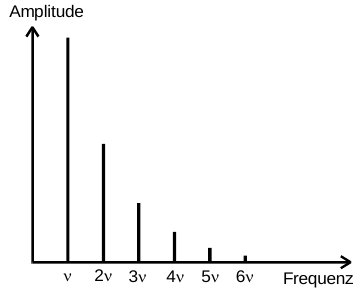
\includegraphics[width=0.6\textwidth]{pics/amplitude_frequenz.jpeg}
\caption{Spektrum einer $v$ periodischen Funktion - Bild aus der Versuchsanleitung entnommen}
\label{pic_spec}
\end{figure} Das Spektrum einer nicht-periodischen Funktion ist kontinuierlich.\\

Wird versucht, eine nicht-stetige Funktion mittels einer Fourierreihe zu entwickeln, so konvergiert diese an der Sprungstelle nicht gegen die Funktion, sondern hat dort eine, mit genauer werdender Approximation größer werdende, endliche Abweichung. Dies wird als Gibbsches Phänomen bezeichnet.

\subsection{Fouriertransformation}
Die Fouriertransformation einer Funktion $f(t)$ bezeichnet das Ausführen folgenden Integrals:
\begin{align}
g(v) = \int \limits _{-\infty}^\infty f(t) e^{ivt} dt
\label{eq_ftrafo}
\end{align}
Dabei stellt die Funktion $g(v)$ das gesamte Frequenzspektrum der Funktion $f(t)$ dar (vlg. Grafik \ref{pic_spec}). Im Falle einer periodischen Funktion sind die so entstehenden $\delta$ Peaks äquidistant und konvergieren gegen 0, damit die Reihe abbricht.\\

Die Fouriertransformation ist auch umkehrbar. So erhält man durch Anwenden des Integrals
\begin{align}
f(t) = \frac{1}{2\pi} \int \limits ^\infty _{-\infty} g(v) e^{-ivt} dv
\label{eq-ruecktrafo}
\end{align}
aus dem Frequenzspektrum wieder die ursprüngliche Funktion.\\

Sollen in der Praxis periodische Signale mit der Fourieranalyse untersucht werden, so erhält man anstelle der scharfen $\delta$ Peaks, stetige und differenzierbare Peaks, da man nicht über eine unendlich lange Zeit (dh. unendlich viele Perioden) integrieren kann. Die Funktion ist somit nur noch auf einem endlichen Bereich periodisch. 

\section{Durchführung}
Mit einem Funktionsgenerator werden periodische Funktionen erzeugt, die dann mittels Fourieranalyse untersucht werden sollen. Das verwendete Messgerät ist ein sog. Analysator. Dieser besteht aus einem Schwingkreis, an den das Signal über einen hochohmigen Widerstand angelegt wird. 
\begin{figure}[htbp]
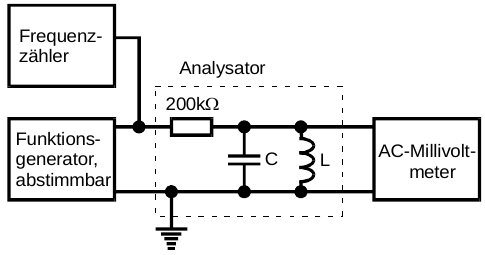
\includegraphics[width=0.6\textwidth]{pics/analysator.jpeg}
\caption{Für den Versuch verwendeter Analysator - Bild aus der Versuchsanleitung entnommen}
\end{figure}

Verändert man die Kapazität und somit die Resonanzfrequenz des Schwingkreises
\begin{align}
v_R=\frac{1}{2\pi\sqrt{LC}},
\end{align}
so beobachtet man beim Resonanzfall eine Spannungszunahme proportional zur Eingangsamplitude. Um die Werte gut am Graphen ablesen zu können, müssen die Resonanzkurven steil abfallen. Verwendet man nur einen Schwingkreis, so fällt diese mit $v^2$ ab. Höhere Potenzen kann man erhalten, indem man mehrere Schwingkreise miteinander kombiniert.
\section{Auswertung}

\section{Diskussion}

% ========================================
%	Literaturverzeichnis
% ========================================

%\bibliographystyle{plainnat}			% Bibliographie-Style auswählen
%\bibliography{BIBDATEI}			% Literaturverzeichnis

% ========================================
%	Das Dokument endent
% ========================================

\end{document}
